\chapter{RDD}

Los Resilient Distributed Datasets, RDD, si atendemos a sus siglas, son colecciones de datos distribuidos, de tipado estático, inmutables y de evaluación perezosa usadas por Spark para realizar trabajos cuyo cometido es ir realizando una sucesión de funciones sobre estos RDD con el fin de obtener un resultado.\\
 
Con estas líneas nos pueden asaltar no pocas cuestiones. ¿A qué tipo de colecciones de datos nos referimos? ¿Dónde se distribuyen? ¿Qué quiere decir que son inmutables? ¿Y de evaluación perezosa? Esclarezcamos esta definición de RDD descomponiéndola para asimilar así mejor su contenido:\\
 
Las colecciones de datos que forman los RDD no son solo cualquier tipo de objeto de Python, Java o Scala, sino que  además pueden ser objetos definidos por el usuario. Los datos que conforman el RDD se dividen en particiones que son repartidas entre los diferentes nodos esclavos del clúster. Con inmutables nos referimos a que son solo de lectura, puesto que no se prestan a modificaciones, dado que los RDD van siendo creados a partir de la transformación de otro RDD, de la distribución de una colección de objetos, como puede ser un array, en el driver o de la lectura de datos en memoria, o bien, en algún otro tipo de almacenamiento. Para finalizar este desglose léxico, atendemos al término “evaluación perezosa”. Con él, afirmamos que los RDD son calculados únicamente cuando los datos finales deben computarse, esto es, cuando sobre ellos recae una acción, como veremos más adelante.\\

\section{RDD de pares clave valor}

Son un tipo especial de RDD, compuestos por pares de clave - valor (key-value), lo cual significa que están formados por una lista de tuplas cuyo primer elemento corresponde a la clave y el segundo es el valor que se le asocia a la clave. Podrían ser comparados, pues, con diccionarios o mapas en otros lenguajes de programación, como Python o Java. Spark habilita muchas funciones específicas para trabajar con este tipo de RDDs, ya que le posibilitan actuar en cada clave en paralelo, o reagrupar datos en la red.\\

\section{Propiedades de los RDD}
Ahora que ya hemos estudiado la definición de los RDDs en general, veamos las cinco propiedades internas que caracterizan un RDD en particular: la lista de objetos de partición, la lista con las dependencias de los RDDs padres, una función, una ubicación y el particionador:

\begin{itemize}
\item La lista de objetos de partición que componen el RDD puede ser consultada mediante la función \textit{partitions()}, que devuelve un array con los objetos de partición, que componen las partes del conjunto de datos distribuidos.
 
\item La lista con las dependencias de los RDDs padres, la cual puede ser consultada mediante la función \textit{dependencies()}. Las dependencias pueden ser de dos tipos: narrow o wide. Las primeras corresponden a particiones que dependen de un pequeño subconjunto de particiones del padre, mientras que las segundas son aquellas en las que la partición ha sido creada mediante una reorganización de todos los datos del padre.
 
\item Una función para calcular los elementos de una partición p, dados iteradores para sus particiones padres \textit{iterator(p, parentIters)}. No es común que un usuario llame directamente a esta función. Lo normal es que sea usada por Spark cuando se calculan acciones.
 
\item Una ubicación preferencial de cada partición. Para consultar la localidad de los datos en una partición p podemos usar la función \textit{preferredLocations(p)}, que devuelve una secuencia de string que nos informa sobre cada uno de los nodos donde se almacena la partición p.
 
\item Un particionador. Mediante la función \textit{partitioner()} obtenemos información acerca de si en el  RDD existe una relación entre los datos y la partición asociada a ellos, como un hashPartitioner. \textit{partitioner()} devuelve un optiontype de Scala, siendo None el resultado en aquellos RDD que no sean de tipo Clave Valor.

\end{itemize}

Las tres primeras en conjunto constituyen la ruta desde un RDD hasta su RDD raíz, se conocen como linaje y suponen que cada partición de los datos contenga la información necesaria para ser recalculada, haciendo a Spark tolerante a fallos. Las otras dos son opcionales y se utilizan como optimizadores.\\

\section{Funciones sobre RDDs}
 
Las operaciones que pueden realizarse sobre RDDs se engloban en dos tipos: transformaciones y acciones.\\
 
Las acciones son aquellas operaciones que devuelven algo que no es un RDD. Devuelven información al driver o escriben datos en sistemas de almacenamiento externo. Dado el carácter perezoso de los RDD, son necesarias para la evaluación de un programa de Spark. Algunas acciones mandan la información al driver, por lo que el resultado de cualquier acción debe caber en su memoria. Por este motivo, es preferible evitar acciones que devuelvan el total de los datos al driver, como \textit{collect()}, y usar en su lugar otras que retornen una cantidad elegida por el usuario, como \textit{first()}, \textit{take(n)}, \textit{count}, etcétera.\\
 
Las transformaciones son las operaciones que tienen como resultado un RDD, suponen el concepto básico de trabajo en Spark y constituyen la mayor parte de la potencia de la API de Spark. Dado que  los RDD  son inmutables y están tipados estáticamente, si intentamos realizar una transformación, por pequeña que sea, en un RDD nuestro RDD original no se verá afectado, lo que obtendremos es un nuevo RDD con una nueva definición de sus propiedades. Además, son calculadas de manera perezosa, por lo que su cómputo será ejecutado cuando al RDD resultante se le aplique una acción. Por lo general, las transformaciones tienen un comportamiento a nivel de elemento, actuando de uno en uno de manera paralela en las diferentes particiones de un RDD.\\
 
Las transformaciones se dividen en dos categorías: transformaciones con dependencias \textit{narrow} y transformaciones con dependencias \textit{wide}. Para un buen desarrollo de aplicaciones en Spark, es de vital importancia entender las diferencias entre estas dos categorías, ya que una aplicación construida sin tenerlas en consideración supondrá un impacto muy negativo a nivel de eficiencia.\\
 
Las transformaciones con dependencias \textit{narrow} son aquellas en las que los datos del RDD padre (el RDD sobre el que se aplica la transformación) no necesitan ser mezclados a nivel de partición para calcular el RDD hijo (el RDD resultante de aplicar la transformación al RDD padre), por lo que pueden ser ejecutadas en un subconjunto de datos sin necesidad de información acerca del resto de particiones. De esta manera, el RDD hijo tendrá un número finito de dependencias en las particiones del RDD padre. Transformaciones que se encuentran en esta categoría son \textit{map}, \textit{flatMap}, \textit{filter}.\\
\begin{figure}[H]
	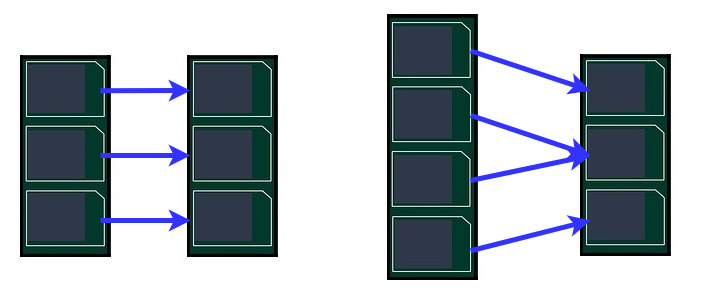
\includegraphics[scale=0.6]{img/narrow}
	\caption{Transformaciones con dependencias narrow}
	\label{foto}
\end{figure}
 
Las transformaciones con dependencias \textit{wide}, por el contrario, son aquellas que requieren un particionado particular de los datos, siendo necesaria la consulta de datos en las distintas particiones del RDD padre, implicando una mezcla en los datos de dichas particiones para computar el RDD hijo; esta operación de compartición de información a través de distintas particiones es conocida en Spark como shuffle, y la estudiaremos detenidamente más adelante. Ejemplos de estas transformaciones son \textit{sort}, \textit{reduceByKey}, \textit{gruoupByKey}.\\
\begin{figure}[H]
	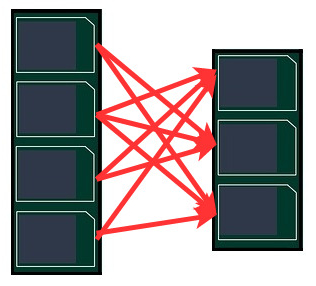
\includegraphics[scale=0.6]{img/wide}
	\centering
	\caption{Transformaciones con dependencias wide}
	\label{foto}
\end{figure}

\section{APIs estructuradas}

Hasta ahora, cuando hemos hablado acerca de las estructuras de datos en Spark lo hemos hecho en términos de RDD. No obstante, hoy por hoy no es la herramienta más utilizada. En este apartado vamos a hablar de los DataFrames y los Datasets, que constituyen las APIs estructuradas de Spark, que son las más usadas en la actualidad.\\

Podemos pensar en los DataFrames y en los Datasets como una tabla distribuida de datos con filas y columnas. El esquema, propiedad inherente a estos, es la lista que define las columnas y los tipos dentro de estas columnas. El usuario puede definirlo, o puede ser leído  por una fuente de datos. Los DataFrames y los Datasets comparten algunas semejanzas con los RDD, como por ejemplo, su inmutabilidad y su evaluación perezosa.\\

\subsection{Datasets}

Están presentes en el ecosistema Spark desde Spark 1.6. Representan conjuntos tipados de datos. En ellos, la comprobación del tipado se realiza en tiempo de compilación. Sólo están disponibles para los lenguajes basados en JVM, es decir, para Scala y para Java, dado que los tipos que admite son los tipos de Java o case class de Scala.\\

\subsection{Los DataFrames} 

Se trata de la API estructurada más usada actualmente y aparecieron en la versión Spark 1.3. Se suele decir que se trata de conjuntos no tipados, lo cual es incorrecto. La comprobación del tipado especificado se realiza en tiempo de ejecución. Internamente, Spark trata a los DataFrames como Datasets de tipo \textit{row}, que permite liberarse de los costes de recolección de basura y creación de instancias de objetos que implican los tipos de JVM. Están disponibles en cuatro lenguajes: Java, Python, Scala y R. 


